\documentclass[10pt,border=4pt]{standalone}
\usepackage{mathptmx}
\usepackage{amsmath,amssymb,bm}
\usepackage{tikz}
\usetikzlibrary{patterns,decorations.pathmorphing,decorations.pathreplacing,arrows.meta,fit,backgrounds,calc,positioning,shapes.geometric}
\definecolor{acc}{HTML}{0B5394}
\definecolor{accl}{HTML}{EAF0F7}
\definecolor{grp}{HTML}{F5F5F5}
\definecolor{org}{HTML}{C55A11}
\definecolor{orgl}{HTML}{FBEFE6}
\tikzset{
 dat/.style={draw=black,line width=0.6pt,fill=white,align=center,font=\small,inner sep=3pt,minimum height=0.85cm},
 lay/.style={draw=acc,line width=0.8pt,fill=accl,rounded corners=2pt,align=center,font=\small,inner sep=3pt,minimum height=0.85cm},
 cnd/.style={draw=org,line width=0.8pt,fill=orgl,rounded corners=2pt,align=center,font=\small,inner sep=3pt,minimum height=0.75cm},
 op/.style={circle,draw=black,line width=0.6pt,fill=white,inner sep=0.5pt,font=\small,minimum size=5mm},
 grpb/.style={draw=black!45,dashed,line width=0.6pt,rounded corners=3pt,inner sep=6pt},
 arr/.style={-{Latex[length=2.2mm,width=1.7mm]},line width=0.7pt},
 carr/.style={-{Latex[length=2.2mm,width=1.7mm]},line width=0.7pt,draw=org},
 shp/.style={font=\scriptsize,text=black!70,inner sep=1pt},
 lab/.style={font=\footnotesize,inner sep=1pt},
 ttl/.style={font=\small\bfseries,inner sep=0pt,anchor=west}
}
\newcommand{\xh}{\mathbf{x}_h}\newcommand{\xf}{\mathbf{x}_f}

\begin{document}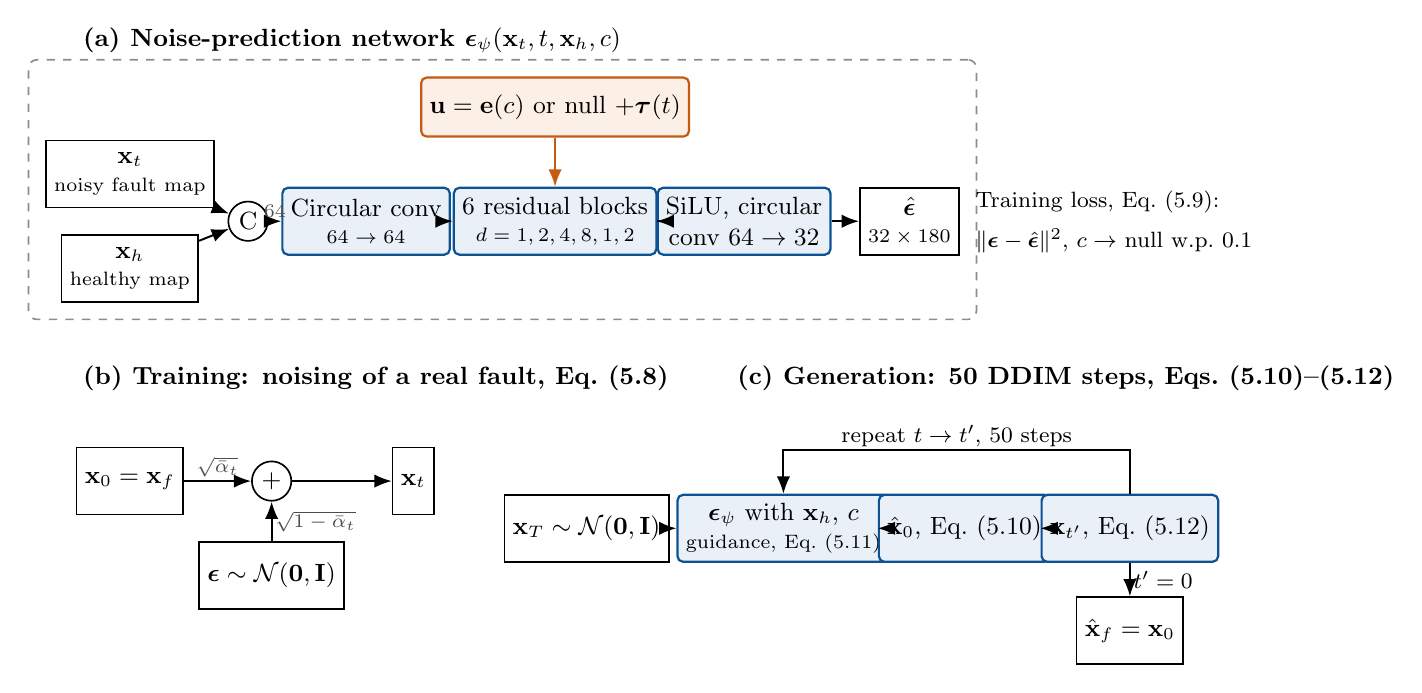
\begin{tikzpicture}[x=1cm,y=1cm]
\node[ttl] at (-0.6,2.3) {(a) Noise-prediction network $\boldsymbol\epsilon_\psi(\mathbf{x}_t,t,\xh,c)$};
\node[dat] (xt) at (0,0.6) {$\mathbf{x}_t$\\[-1pt]\scriptsize noisy fault map};
\node[dat] (xh) at (0,-0.6) {$\xh$\\[-1pt]\scriptsize healthy map};
\node[op] (cat) at (1.5,0) {C};
\node[lay] (s1) at (3.0,0) {Circular conv\\[-1pt]\scriptsize $64\to64$};
\node[lay] (b1) at (5.4,0) {6 residual blocks\\[-1pt]\scriptsize $d=1,2,4,8,1,2$};
\node[lay] (o1) at (7.8,0) {SiLU, circular\\conv $64\to32$};
\node[dat] (eps) at (9.9,0) {$\hat{\boldsymbol\epsilon}$\\[-1pt]\scriptsize $32\times180$};
\draw[arr] (xt)--(cat); \draw[arr] (xh)--(cat); \draw[arr] (cat)--node[shp,above]{64}(s1); \draw[arr] (s1)--(b1); \draw[arr] (b1)--(o1); \draw[arr] (o1)--(eps);
\node[cnd] (u) at (5.4,1.45) {$\mathbf{u}=\mathbf{e}(c)$ or null $+\boldsymbol\tau(t)$}; \draw[carr] (u)--(b1);
\node[lab,align=left,anchor=west] at (10.7,0.25) {Training loss, Eq.~(5.9):};
\node[lab,align=left,anchor=west] at (10.7,-0.25) {$\lVert\boldsymbol\epsilon-\hat{\boldsymbol\epsilon}\rVert^2$, $c\to$ null w.p.\ 0.1};
\begin{scope}[on background layer]\node[grpb,fit=(xt)(xh)(eps)(u)] {};\end{scope}
% (b) forward noising and sampling
\node[ttl] at (-0.6,-2.0) {(b) Training: noising of a real fault, Eq.~(5.8) \qquad (c) Generation: 50 DDIM steps, Eqs.~(5.10)--(5.12)};
\node[dat] (x0) at (0,-3.3) {$\mathbf{x}_0=\xf$};
\node[op] (no) at (1.8,-3.3) {$+$};
\node[dat] (xtt) at (3.6,-3.3) {$\mathbf{x}_t$};
\draw[arr] (x0)--node[shp,above]{$\sqrt{\bar\alpha_t}$}(no); \draw[arr] (no)--(xtt);
\node[dat] (ep) at (1.8,-4.5) {$\boldsymbol\epsilon\sim\mathcal{N}(\mathbf{0},\mathbf{I})$}; \draw[arr] (ep)--node[shp,right]{$\sqrt{1-\bar\alpha_t}$}(no);
\node[dat] (xT) at (5.8,-3.9) {$\mathbf{x}_T\sim\mathcal{N}(\mathbf{0},\mathbf{I})$};
\node[lay] (net) at (8.3,-3.9) {$\boldsymbol\epsilon_\psi$ with $\xh$, $c$\\[-1pt]\scriptsize guidance, Eq.~(5.11)};
\node[lay] (x0h) at (10.6,-3.9) {$\hat{\mathbf{x}}_0$, Eq.~(5.10)};
\node[lay] (up) at (12.7,-3.9) {$\mathbf{x}_{t'}$, Eq.~(5.12)};
\node[dat] (out) at (12.7,-5.2) {$\hat{\mathbf{x}}_f=\mathbf{x}_0$};
\draw[arr] (xT)--(net); \draw[arr] (net)--(x0h); \draw[arr] (x0h)--(up);
\draw[arr] (up.north) -- ++(0,0.55) -| node[lab,above,pos=0.25]{repeat $t\to t'$, 50 steps} (net.north);
\draw[arr] (up)--node[lab,right]{$t'=0$}(out);
\end{tikzpicture}\end{document}
